% !TeX root = ../master.tex

\lecture{2}{2026-08-27}{Fibermaterialer, pt. II}
Typisk vil høj-styrke kulfiber være produceret af PAN mens høj-modulus typisk kommer af \textit{pitch}.
I produktionen af specielt kulfibre er begrebet \textit{sizing} vigtigt.
Sizing referer til den overfladebehandling man giver fibrene for at de kan binde til matrixmaterialet.
Ikke-sizet kulfiber vil typisk være yderst resistent mod at binde til et matrixmateriale således at det ikke i sig selv er egnet til at lave kulfiber af.
Glasfiber sizes normalt også omend dette er en meget anden process end hvad gør sig gældende for kulfiber qua de forskellige materialekemier.

På \Mref{fig:carbon-fiber} ses en kulfiber forstørret op.
Her ses en masse cavities mellem de mange kulfiberplader.
Idet fiberen strækkes, bliver de her cavities ``presset sammen'' idet pladerne trykkes mod hinanden og alignes.
Dette hindrer bevægelsen af dislokationer således at materialet bliver stærkere/stivere.

\begin{figure} [ht]
  \centering
  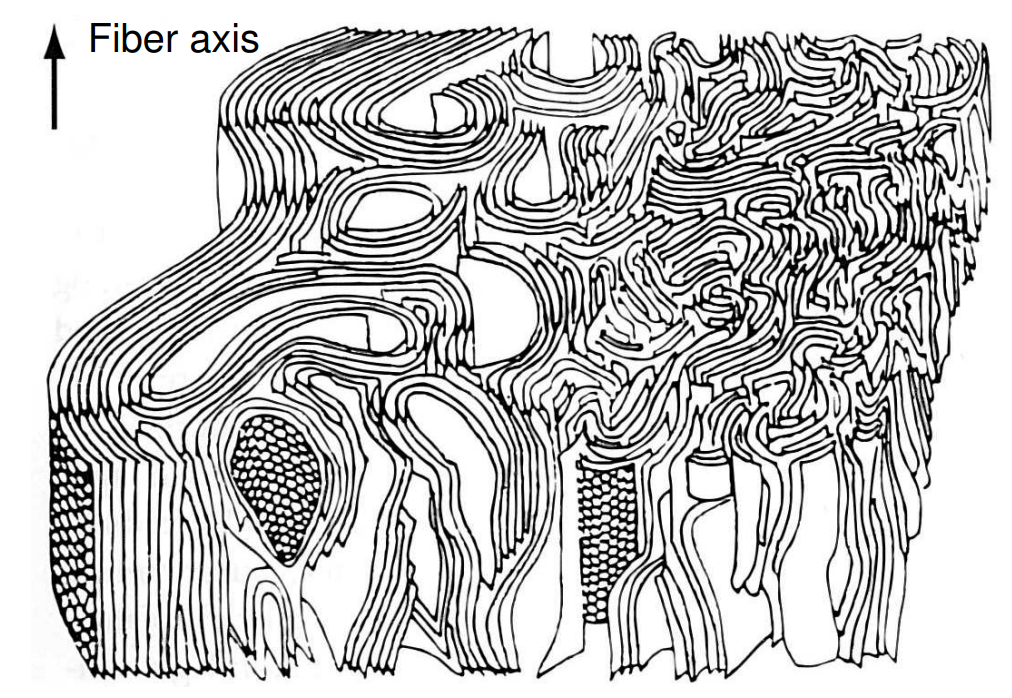
\includegraphics[width=0.6\linewidth]{./figures/carbon-fiber.png}
  \caption{Skematisk repræsenation af strukturen af en kulfiber. Reproduceret fra \citepage{hull2007introductioncompositematerials}{Fig. 2.1}, originalt fra \cite{bennett1978structuralcarbonfibres}.}
  \label{fig:carbon-fiber}
\end{figure}


\subsection{Aramidfibre}
Aramidfibre er typisk gule og kommer fra aramid-polymeren der spindes op til fibre.
Blandt aramiderne er bl.a. handelsnavnene Kevlar (skudsikre veste), Nomex (brandhæmmende dragter), Technora, osv.
Aramidfibre er typisk omtrent så stive som glasfiber, men begge overgås klart af kulfiber.
Styrkemæssigt er aramid typisk svagere end både glasfiber og kulfiber.
Slag-sejheden for aramidfibre er dog væsentligt højere end både hvad gælder kul- og glasfiber.
